\documentclass[11pt,a4paper]{article}
\usepackage{od}
\usepackage[utf8]{inputenc}
\usepackage[russian,main=ngerman]{babel}

\title{Über die Gesetze der Konstruktion technischer Systeme }

\author{B.I.Goldovsky}
\date{Februar 2018}

\begin{document}
\maketitle
\begin{quote}
  Original: \foreignlanguage{russian}{О законах построения технических
    систем}\footnote{\url{https://www.metodolog.ru/node/2164}.}.

  Erschienen in \foreignlanguage{russian}{ТРИЗ нужна России: проблемы
    технического творчества. Сб. ст. выпуск 2. – Чебоксары: Новое время, 2018.}
  S. 54 - 72.
  
  Übersetzt von Hans-Gert Gräbe, Leipzig, mit Unterstützung durch die freie
  Version von \texttt{deepl.com}.
\end{quote}

Die von G.S.Altshuller [1] vorgeschlagene Liste der Gesetze der Entwicklung
technischer Systeme (TS) ist relativ künstlich und bedingt unterteilt in die
Gesetze der „Statik“, der „Kinematik“ und der „Dynamik“. Ein Schritt in
Richtung einer natürlichen Klassifizierung dieser Gesetze wurde in den frühen
1980er Jahren von V.M. Petrov vorgenommen, der die Gesetze der „Statik“ als
„Organisations-Gesetze“ bezeichnete (d.h. Gesetze der Konstruktion), die
Gesetze der „Kinematik“ und „Dynamik“ dagegen zu „Evolutionsgesetzen“
(d.h. Entwicklungsgesetzen) vereinigte [2], [3] (unter Verwendung von seinen
frühen Ausarbeitungen zu diesem Thema). Fast zur gleichen Zeit hat auch der
Autor dieses Aufsatzes Ausarbeitungen zur Entwicklung eines Systems von
Gesetzmäßigkeiten der Konstruktion und Entwicklung technischer Systeme
vorgelegt [4]. Ziel dieser Ausarbeitungen war einfach, das Thema zu verstehen.
Dabei wurden drei wesentliche Momente angemerkt:
\begin{itemize}
\item Das System der Gesetzmäßigkeiten ist in Wirklichkeit viel komplexer als
  die in [1] aufgeführte Liste.
\item Ein Teil der Gesetzmäßigkeiten lässt sich deduktiv begründen.
\item Im System der Gesetzmäßigkeiten ist es notwendig, die Gesetze der
  Konstruktion TS herauszuheben, welche die Arbeitsfähigkeit des TS sichern,
  weil die Gesetze der Entwicklung im Rahmen der Gesetze der Konstruktion
  wirken.
\end{itemize}

Die letzte These, als methodologisch wichtig, wurde 1983 in den
Konferenzthesen [5] veröffent\-licht (siehe auch [6]). Es gab auch Versuche,
in späteren Publikationen darauf aufmerksam zu machen, aber ohne Erfolg. Das
ist durchaus verständlich, denn die Hauptarbeiten der TRIZ-Spezialisten zu
Gesetzen der Konstruktion und Entwicklung technischer Systeme konzentrierten
sich hauptsächlich auf die Beschreibung der Gesetzen, ihre Klassifizierung und
Untersetzung mit Beispielen [7], [8]. Die Frage der Mechanismen der
Funktionsweise der Gesetze, wofür diese methodologische These wichtig sein
könnte, wurde nicht untersucht.

\begin{emph}
  Ein solches Phänomen ist ganz typisch für die Entwicklung jeder
  wissenschaftlichen Erkenntnis. Wie in [9] erwähnt wird: „Die Wissenschaft
  bewegt sich wie mit dem Rücken zur Zukunft; sie drängt vorwärts und lässt
  uns den zurückgelegten Weg überblicken. Wer sich schneller bewegt und seine
  Zeitgenossen überholt, fällt aus dem Gesichtsfeld“.
\end{emph}

Im Jahr 2017 bezeichnete N.A. Shpakowski in [10], unter Anwendung des Systems
der Gesetze von V.M. Petrov auf den Prozess der Schaffung und Entwicklung TS,
die Gesetze der Organisation als zentrale und die Gesetze der Evolution als
unterstützende. Eine solche Einteilung ist nicht ganz korrekt, da diese
Gesetze in unterschiedlichen Bereichen wirken. Doch der Fakt der Hervorhebung
der besonderen Rolle der Gesetze der Konstruktion TS selbst ist richtig. Worin
besteht aber die Besonderheit der Gesetze der Konstruktion TS?

Es ist bekannt, dass alle TS Teil von zwei Beziehungssystemen sind: der Natur
und der Gesellschaft (des menschlichen Soziums).  Sie werden vom Sozium für
die Bedürfnisse des Menschen geschaffen, aber unter Verwendung des natürlichen
Substrats.  In Bezug auf die technischen Widersprüche wurde dies in [11]
gezeigt: Die Beziehungen der gegenseitigen Bedingtheit der Parteien des
Widerspruchs sind durch das natürliche Substrat bestimmt (daher sind diese
Beziehungen bedingungslos -- \foreignlanguage{russian}{безусловно}), und die
Beziehungen der Gegensätzlichkeit werden durch Bewertungen durch das Sozium
bestimmt (und sind daher relativ, nicht bedingungslos). Ein ähnliches Bild
ergibt sich auch in Bezug auf die Gesetze der Konstruktion und Entwicklung TS.

Es sei angemerkt, dass ein Gesetz eine Zwangskategorie ist. Jedes
bedingungslose Gesetz wird die Nichteinhaltung seiner Anweisungen bestrafen.
In dieser Hinsicht unterscheiden sich die Gesetze der Konstruktion TS
erheblich von den Entwicklungsgesetzen (sowohl in ihrem Wesen als auch ihrem
Wirkmechanismus). Die Gesetze der Konstruktion TS sind als Reflexion des
natürlichen Substrat der Technik bedingungslos: ihre Verletzung führt
unmittelbar zur Funktionsunfähigkeit des TS (d.h. die Bestrafung für ihre
Verletzung ist unvermeidlich). Die Gesetze der Entwicklung spiegeln den
Einfluss des Soziums auf die Technik wider und sind, genau wie die Gesetze des
Soziums, nicht bedingungslos. Ihre Verletzung führt nicht zu einer sofortigen
Bestrafung, führt die Entwicklung des TS aber von einer optimalen Bahn.
\emph{Daher ist die Identifizierung eines Mechanismus, der erzwingt, dass den
  Gesetzen der Entwicklung TS bei deren Verbesserung zu folgen ist, eine recht
  schwierige Aufgabe, mit der man sich beschäftigen muss}. Gleichzeitig macht
die bedingungslose Wirkung der Gesetze der Konstruktion TS diese invariant
gegenüber allen Transformationen eines TS.  Dementsprechend können sie
verwendet werden, um die Richtigkeit der Transformationen zu kontrollieren
und, wie jede wesentliche Einschränkung, auf den Wirkmechanismus der Gesetze
der Entwicklung TS einwirken.

Diese Ausführungen gehören zu den theoretischen Kenntnissen, die, im Gegensatz
zu angewandten, bei der Mehrheit der TRIZ-Spezialisten nicht gefragt sind (so
der Autor in [12]).  In konkreten Anwendungen werden die Gesetze der
Konstruktion TS in erster Linie bei der Synthese TS eingesetzt.  Allerdings
sind sie auf Grund ihrer hohen Allgemeinheit den zahlreichen gesetzmäßigen
Regeln der Konstruktion arbeitsfähiger TS unterlegen, die das Wesen der
Ingenieursdisziplinen in verschiedenen Bereichen der Technik ausmachen.
Gleichzeitig macht gerade der allgemeine Charakter der Gesetze der
Konstruktion TS sie hinreichend universell.  Wobei einzelne Schlussfolgerungen
aus diesen Gesetzen einen eigenständigen Anwendungswert haben.

Die Gesetze der Konstruktion TS sind in unterschiedlichem Detaillierungsgrad
in vielen Quellen beschrieben, zum Beispiel in [7], [13], [14], [15], [16],
[17]. Dennoch erscheint es angebracht, dieses Thema unter Berücksichtigung der
in den verschiedenen Jahren geleisteten Arbeit kompakt zu umreißen.

Der wichtigste systembildende Faktor für ein TS ist seine primär nützliche
Funktion (PNF), die einem Bedürfnis des Soziums entspricht. Die Umsetzung der
PNF erfordert ihrerseits die Ausführung einer Reihe von Funktionen auf
niedrigerer Ebene von Allgemeinheit, von elementaren nützlichen Funktionen
(ENF).  Zum Beispiel müssen für Fahrzeuge mit PNF „Transport von Fracht auf
der Wasseroberfläche“ die folgenden ENFs umgesetzt werden:
\begin{itemize}[noitemsep]
\item Gewährleistung von Platzierung und Fixierung der Ladung während des
  Transports;
\item Sicherstellung der Haltens des Transportmittels auf der
  Wasseroberfläche;
\item Sicherstellung der Bewegung des Transportmittels auf der
  Wasseroberfläche;
\item Steuerung der Bewegung des Transportmittels.
\end{itemize}
Zur Realisierung der ENF im System müssen entsprechende Subsysteme vorgesehen
werden. D.h.  es muss die \textbf{funktionale Vollständigkeit des TS}
gewährleistet sein: im System müssen alle Teilsysteme realisiert sein, die zur
Ausführung der PNF erforderlich sind.

Die angegebenen ENFs bilden die erste Ebene der Zerlegung der PNF, ihre
Zusammensetzung bleibt bei jeder Änderung der Wirkprinzipien der einzelnen
Teilsysteme unverändert. Diese Stabilität der Zusammensetzung der ENF der
ersten Ebene und der entsprechenden Subsysteme des TS macht sie zu einer
Invarianten und zu einem Marker einer bestimmten Gruppe (Klasse) von
technischen Mitteln, die in eine bestimmte \textbf{funktionelle Nische}
entsprechend der PNF fallen.

Die Ausführung der PNF und der entsprechenden ENFs wird durch die Struktur der
TS gewährleistet als Elemente des natürlichen Substrats, die auf eine
bestimmte Art und Weise miteinander interagieren.  Gerade daraus ist
zurückzuführen, dass bei der Interaktion der Elemente nicht alle ihre
Eigenschaften realisiert werden, sondern nur einige, und dass sich durch die
bestimmte Kombination von Eigenschaften bei der Interaktion eine spezielle
Systemeigenschaft herausbildet, die nicht auf die Summe der Eigenschaften der
in der Struktur enthaltenen Elemente reduzierbar ist.  Gleichzeitig erzeugt
die aber auch einen strukturellen Überschuss im TS [18].

Die Anzahl und Zusammensetzung der Elemente, die in der Struktur enthalten
sind, stimmt nicht mit der Anzahl und Zusammensetzung der funktionalen
Subsysteme überein, da einige Elemente Teil mehrerer Subsysteme sein können.

Die funktionale Vollständigkeit des TS muss der \textbf{strukturellen
  Vollständigkeit} des Systems entsprechen, die besagt, dass die
Zusammensetzung der Elemente und die Wechselwirkungen zwischen ihnen
ausreichen müssen, um alle zum System gehörenden Elementarfunktionen ausführen
zu können.  Deshalb ist es zweckmäßig, das Funktionieren als Prozess
geeigneter Transformationen natürlichen Flüsse (von Stoffen, Energie und
Information) darzustellen. Derartige Darstellung entsprechen einem aus der
Kybernetik bekannten Strukturierungsansatz, der aus einem Umformer (Black Box)
mit Ein- und Ausgängen besteht (wobei über einen der Eingänge die Steuerung
erfolgen kann). Der Ansatz der Darstellung des Funktionierens durch
Transformation von Flüssen wird z.B. in der bekannten Arbeit von R. Koller
[19] aufgenommen.

Nach dieser Darstellung kann das \textbf{Gesetz der strukturellen
  Vollständigkeit eines TS} wie folgt formuliert werden: \textbf{Die
  Gesamtheit der Elemente der Struktur und die Wechselwirkungen zwischen ihnen
  müssen den Durchsatz der natürlichen Flüsse (Stoff, Energie und/oder
  Information) zu den notwendigen Teilen des Systems sichern sowie eine solche
  Umwandlung dieser Ströme, dass alle elementaren Funktionen des Systems
  erfüllt werden}.

Die angeführte Definition bezieht sich auf die so genannten dynamischen
Systeme (Maschinen, Geräte und Apparate), in denen für den Menschen
lebensnotwendige natürliche Prozesse realisiert werden, die das Funktionieren
eines TS gewährleisten. Es gibt jedoch auch Anlagen
(\foreignlanguage{russian}{сооружение}), die gemeinhin als statisch betrachtet
werden.  In [16] wurde allerdings gezeigt, dass eine Einteilung in statische
und dynamische Systeme in gewisser Weise bedingt ist.  Wenn man jedoch von der
Wesentlichkeit oder Unwesentlichkeit dynamischer Prozesse als Unterscheidung
ausgeht, lassen sich Anlagen von Maschinen, Geräten und Apparaten
unterscheiden.  In [13] wurde gezeigt, dass man auch in Anlagen Analoga von
Flüssen finden kann als Bild der Verteilung von Spannungen und/oder
Verformungen.  Zum Beispiel kommt das Bild der Spannungsverteilung in einer
Metallplatte mit variablem Querschnitt mit Kerben und Mulden bei Dehnung dem
Bild der Geschwindigkeitsverteilung in der Strömung einer nichtviskosen
Flüssigkeit in einer Rohrleitung mit einer ähnlichen Querschnittsänderungen
sehr nahe. Ähnliche Details ergeben sich bei der Untersuchung von Hindernissen
für Flüsse.  Das heißt, im Prinzip kann der Fluss-Ansatz auch auf Anlagen
angewendet werden. Dementsprechend kann auch der Begriff der strukturellen
Vollständigkeit auf Anlagen angewendet werden.

\begin{emph}
  In der TRIZ wurde der Fluss-Ansatz zuerst von Yu.I. Khotimlyansky [20]
  vorgeschlagen. Bezogen auf Energieflüsse wurde das Prinzip des
  Energiedurchsatzes vorgeschlagen („notwendige Voraussetzung für des Betrieb
  eines TS ist der Energiedurchsatz durch alle Objekte des Systems“).  Weiter
  wurde vorgeschlagen, zwei Arten der Energieumwandlung (nach der Art und nach
  den Programm (parametrisch)) zu unterscheiden.  Dies vereinfachte in
  bekannter Weise die Modellierung von Flüssen im Gegensatz zum Ansatz von
  R. Koller, der eine Liste von 12 Gruppen  physikalischer
  Elementarfunktionen vorschlug, von denen jede eine direkte und eine inverse
  Funktion umfasste.
\end{emph}

\begin{emph}
  Es sei angemerkt, dass in Ingenieuraufgaben die Konstruktion von
  integrierten Flussstrukturen (insbesondere in sehr frühen
  Entwicklungsstadien) keine Seltenheit ist. Zum Beispiel werden auf einem
  U-Boot elektrische Akkumulatoren und Druckluft als Energiequellen
  eingesetzt.  Die Verbraucher elektrischer Energie benötigen Strom
  unterschiedlicher Art (Gleich- und Wechselstrom mit unterschiedlichen
  Spannungswerten).  Auch die Verbraucher von Druckluft benötigen einen
  Luftstrom mit verschiedenen Drücken (Hoch-, Mittel- und Niederdruck).
  Darüber hinaus benötigen einige Verbraucher einen Fluss unter Druck
  stehender Hydraulikflüssigkeit, für deren Erzeugung elektrische Energie und
  Druckluft verwendet wird. Es ist auch notwendig, im Apparat Meerwasser zu
  bewegen.  Natürlich wird man ein vergröbertes strukturelles Schema auf der
  Basis der Vorstellungen über Umformer und Black Boxes mit Ein- und Ausgängen
  ausarbeiten, um sich alle erforderlichen Flüsse und Energie-Transformationen
  anschaulich vorzustellen. Mit dieser Art von Erfahrung und basierend auf dem
  vorgeschlagenen Ansatz Yu.I. Khotimlyansky gelang es, als Teil der
  Komplexmethode der Suche nach neuen technischen Lösungen einen ausreichend
  ganzheitlichen Apparat zur strukturellen Synthese und Transformation zu
  entwickeln, mit dem isch auch die Stoff-Feld-Analyse ersetzen ließ [21],
  [13].  Dabei wurden Energie-Ketten modelliert, da sowohl Materie- als auch
  Informationsströme eine Energiekomponente umfassen.
\end{emph}

Das Gesetz der strukturellen Vollständigkeit in der Flussdarstellung vereint
zwei der traditionellen Gesetze der Konstruktion TS, das Gesetz der
„Vollständigkeit“ und das der “Energieleitfähigkeit“, siehe [1]. Es sei darauf
hingewiesen, dass die Formulierung dieser Gesetze faktisch Spezialfällen
entspricht. In der Realität ist das Bild komplexer. Die Zusammensetzung der
Struktur hängt, selbst in verallgemeinerter Form, weitgehend von ihrer
Bestimmung ab. Typische verallgemeinerte Funktionsstrukturen (für Maschinen,
Informationssysteme und Anlagen) sind z.B. in [17] angegeben. Beispiele von
Energieketten verschiedener Bestimmung werden in [13] vorgestellt.

Den größten Einfluss auf die Struktur des Systems haben die
\textbf{Wirkprinzipien} der Teilsysteme, d.h.  jene natürlichen Prozesse,
Effekte und Erscheinungen, deren Gesamtheit die Ausführung der nützlichen
Systemfunktionen absichert. Das Wirkprinzip kann nicht auf der Grundlage der
Funktion bestimmt werden, wenn diese allein auf einer qualitativen Ebene
formuliert ist. Wie oben gezeigt, umfasst die funktionale Nische eine Reihe
von technischen Systemen, die sich in ihren Wirkprinzipien unterscheiden.  Zur
Konkretisierung müssen neben der qualitativen Beschreibung der Funktion auch
deren quantitativen Charakteristika (Parameter) angegeben werden. Mit anderen
Worten, eine funktionale Nische kann in eine Anzahl kleinerer
\textbf{funktionell-parametrischer Nischen} unterteilt werden, in denen sich
jeweils ein spezifisches TS mit seinen eigenen quantitative Parametern und
entsprechenden Wirkprinzipien der Teilsysteme [13] befindet.

\begin{emph}
  Es sei darauf hingewiesen, dass die Berücksichtigung quantitativer Parameter
  TS nur am Rande der TRIZ erfolgt. Es ist vollkommen verständlich, da in
  erfinderischen Formulierungen quantitative Indikatoren meist fehlen.
  Allerdings kann bei einem solchen Verhältnis zu Quantitäten in der TRIZ das
  Gesetz des Übergang von quantitativen zu qualitativen Veränderungen faktisch
  nicht angewendet werden, obwohl es in Veröffentlichungen über die Gesetze
  der Entwicklung TS genannt wird (siehe z.B. [7]). Entsprechend fallen
  Kategorien wie, zum Beispiel, Wesentlichkeit und die Zuspitzung von
  Widersprüchen aus der Praxis heraus.
\end{emph}
Die Nischenvorstellung der Wirkprinzipien TS ist nicht selten.  In [13] wird
zum Beispiel die Verteilung der Wirkprinzipien von Transportmitteln nach
Nischen entsprechend der Geschwindigkeits- und Gewichtsparameter gezeigt.
Ähnliche Abhängigkeiten sind in den Abb. 1 und 2 für elektrische Akkumulatoren
dargestellt.
\begin{center}
  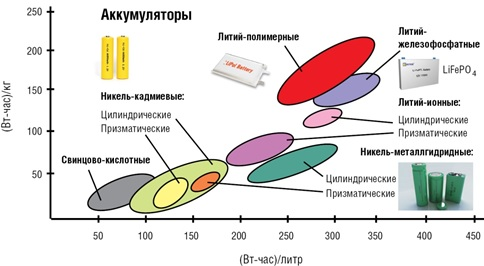
\includegraphics[width=.7\textwidth]{2164-1.jpg}
  \begin{quote}
    Abb. 1 -- Verteilung der verschiedenen Typen von elektrischen
    Akkumulatoren auf Nischen nach den Parametern spezifische Energie pro
    Massen und Volumeneinheit.
  \end{quote}
\end{center}

\begin{center}
  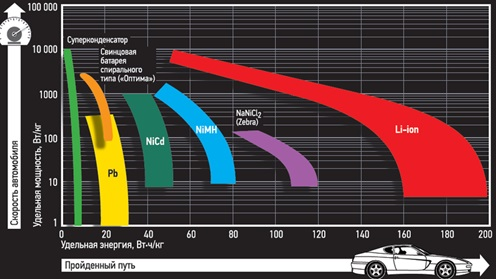
\includegraphics[width=.7\textwidth]{2164-2.jpg}
  \begin{quote}
    Abb. 2 -- Verteilung der verschiedenen Typen von elektrischen
    Traktionsbatterien (Akkumulatoren elektrischer Energie) auf Nischen nach
    den Parametern spezifische Leistung und spezifische Energie pro
    Masseneinheit
  \end{quote}
\end{center}
Eine ähnliche Verteilung auf Nischen haben auch Baumaterialien. Zum Beispiel
ist in Abb. 3 die Abhängigkeit der Materialverteilung für Gefäße auf
entsprechende parametrische Nischen dargestellt.
\begin{center}
  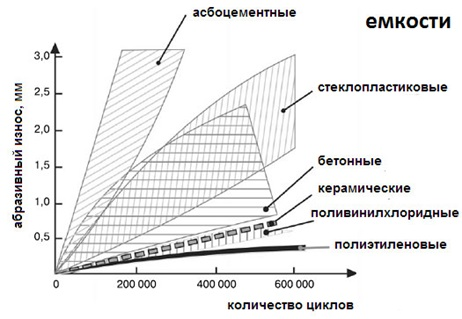
\includegraphics[width=.7\textwidth]{2164-3.jpg}
  \begin{quote}
    Abb. 3 -- Verteilung der verschiedenen Materialtypen für Gefäße auf
    Nischen nach den Parametern zulässiger abrasiver Verschleiß und Anzahl der
    Lastzyklen
  \end{quote}
\end{center}
Damit kann man davon ausgehen, dass sich für Anlagen die Änderung des
Materials faktisch analog der Änderung des Wirkprinzips auswirkt.

Im Gegensatz zur Funktion (PNF, ENF), die ein Spiegel der Ziele (Bedürfnisse)
des Soziums ist, bezieht sich das Wirkprinzip auf das natürliche Substrat als
Mittel zur Ausführung einer Funktion.  Daher ist es zweckmäßig, TS als eine
bestimmte Art von technischen Mitteln (ähnlich einem biologischen Typ) zu
definieren, als Kombination (Einheit) der PNF und des Wirkprinzips des
wichtigsten (zentralen) Subsystems. Unter letzterem wird ein solches Subsystem
verstanden, dessen ENF diejenige Gruppe (Klasse) von TS charakterisiert,
welche die gemeinsame PNF realisieren und sich so von ähnlichen Systemen
unterscheiden.  \emph{Zum Beispiel wird für Systeme mit der PNF, „Realisierung
  des Transports von Gütern auf der Wasseroberfläche“ das grundlegende
  (zentrale) Untersystem ein Untersystem sein, das die ENP „das Fahrzeug auf
  der Wasseroberfläche halten“ sichert, da die übrigen ENPs für fast alle TS
  typisch sind, die Lasten transportieren}.

Eine Nischendarstellung der Wirkprinzipien ist recht nützlich, erstens, weil
sie ein ziemlich vollständiges Bild der realen Möglichkeiten dieser oder jener
technologischer Effekte gibt.  Zweitens erfordert die Arbeit mit
funktional-parametrischen Nischen die Heraushebung der wirklich wesentlichen
Parameter, die die Möglichkeiten der Wirkprinzipien zur Funktionsausführung
quantitativ charakterisieren. Drittens, wenn die Ursache eines erheblichen
unerwünschten Effekts (UE) die Veränderung eines quantitativen Indikators ist,
der eine Nischengrenze definiert, dann ist es am wahrscheinlichsten, dass es
notwendig ist, das Wirkprinzip zu ändern (d.h. zu einem neuen Typ von TS
überzugehen).

Quantitative Charakteristika des Funktionierens sind nicht weniger wichtig wie
qualitative.  Wenn die Bedingungen für die Anwendung eines TS für das Sozium
in Bezug auf das Funktionieren verallgemeinert werden, die zum Beispiel in
[13], [15] und [22] angeführt werden, erhalten wir die folgende Sammlung von
Bedingungen:
\begin{itemize}[noitemsep]
\item Die primär nützliche Funktion (PNF) des TS muss qualitativ (inhaltlich)
  und quantitativ den Anforderungen des Soziums und/oder des technischen
  Umfelds entsprechen.
\item Die Stabilität des Funktionierens muss gewährleistet sein
  (einschließlich der Zuverlässig\-keit des Funktionierens und der
  Widerständigkeit gegenüber äußeren Einflüssen).
\item Der erforderliche Grad der Steuerbarkeit des Prozesses des
  Funktionierens muss gewähr\-leistet sein.
\item Die Benutzerfreundlichkeit der menschlichen Interaktion mit dem TS
  (einschließlich der Benutzerfreundlichkeit der Steuerung) muss gewährleistet
  sein, wenn eine solche Interaktion vorgesehen ist.
\end{itemize}

In den Fällen, in denen eine Weiterentwicklung eines früher erschaffenen und
bereits arbeitenden TS stattfindet, werden die quantitativen Charakteristika
des Funktionierens sozusagen im Arbeitszustand festgelegt, auf der Basis der
Analyse der Bedürfnisse des Soziums und des technischen Umfelds. In den
Fällen, in denen ein TS zum ersten Mal entsteht (Pionier-Entwicklung), ist es
nützlich, sich der Überwindung \textbf{parametrischer Schwellenwerte} zu
erinnern, welche die Arbeitsfähigkeit des Systems charakterisieren [13].  Ein
\textbf{physikalischer} parametrischer Schwellenwert bestimmt die Bedingungen
für das zuverlässige Funktionieren des Systems.  \emph{Zum Beispiel sollte der
  maximale Wert der erzeugten Auftriebskraft 10-20\% das Gewicht eines
  Flugzeugs um 10-20\% überschreiten, damit dieses zuverlässig fliegt. Und bei
  jedem Überwasserschiff mit voller Ladung muss ein Teil des Rumpfes über
  Wasser bleiben, um die Lebensfähigkeit des Schiffes unter verschiedenen
  äußeren Einflüssen zu gewährleisten}. Eine \textbf{funktionelle}
parametrische Schwelle bestimmt dasjenige Niveau der quantitativen Parameter
des Funktionierens, bei dem das geschaffene TS nicht mehr nur als Prototyp
angesehen werden. \emph{Zum Beispiel wird ein Flussdampfer ein echtes
  Transportmittel, wenn er mit einer Tankfüllung gegen den Strom mindestens
  die Entfernung zwischen zwei Anlegestellen zurücklegen kann. Und der
  Überflug von Blériot über den Ärmelkanal (1909) war ein klares Zeichen
  dafür, dass das Flugzeug in die Reihe der einsatzfähigen Transportmittel
  aufgenommen war}.

Eine der grundlegenden gesetzmäßigen Bedingungen der Arbeitsfähigkeit eines TS
ist die Sicherung eines bestimmten \textbf{minimal erforderlichen Maßes an die
  Abstimmung der Struktur des TS}. In [14] wurde gezeigt, dass strukturelle
Kohärenz eine unverzichtbare Systemeigenschaft ist.  Nicht abgestimmte Systeme
sind nicht arbeitsfähig. Dabei wurde vorgeschlagen, den Prozess der Abstimmung
eines TS in zwei Etappen zu teilen: in die Anfangsetappe, in der die
Arbeitsfähigkeit hergestellt wird, die „\textbf{Schwellenabstimmung}“, und
weiter die „\textbf{Optimierungsabstimmung}“. Die Schwellenabstimmung ist
endlich in der Zeit (sie gilt als erfüllt, wenn die Betriebsfähigkeit des TS
erreicht ist), und die quantitative Bedingungen der Schwellenabstimmung haben
die Form von Ungleichungen (“nicht weniger als“, „nicht mehr als“).  Die
Optimierungsabstimmung kann sich über den gesamten Lebenszyklus der TS
erstrecken und die quantitativen Bedingungen der Optimierungsabstimmung haben
die Form von Gleichungen (Gleichsetzungen). Um den vielschichtigen Begriff
„Abstimmung“ nicht überzustrapazieren, kann der anfängliche Prozess der
(Schwellen-)Abstimmung mit dem Begriff „\textbf{Konjugation}“
(\foreignlanguage{russian}{сопряжение}) bezeichnet werden, der in der
Evolutionsbiologie verwendet wird [23]. Bei der Verwirklichung der Konjugation
Implementierung werdenzwingend Struktur und Funktion abgestimmt, wie auch die
Interaktion der Elemente der Struktur untereinander, qualitativ und
quantitativ.

Als Ergebnis der Konjugation wird die \textbf{Konformität von Struktur und
  Funktion} der TS gesichert, was ein ziemlich wichtiges bedingungsloses
Gesetz der Konstruktion ist. Es sei angemerkt, dass dieses Gesetz in [17] als
“Entsprechung von Funktion und Struktur“ formuliert ist, wobei auf den
Nachweis der Objektivität dieser Entsprechung besondere Aufmerksamkeit
gerichtet wird. Diese Tatsache lässt sich dadurch erklären, dass der Übergang
von der Funktion zur Struktur, wie bei jedem Übergang vom Ziel zum Mittel, ein
Verfahren der Synthese ist, das im Prinzip nicht zu einem eindeutigen Ergebnis
führt. Ein eindeutiger Übergang von der Funktion zur Struktur ist nur in
trivialen (stereotypen) Fällen möglich und bei der Suche nach neuen Lösungen
praktisch nicht anzutreffen. Gleichzeitig ist der Übergang von der Struktur
zur Funktion ein analytisches Verfahren mit einem eindeutigen Ergebnis: Wie
die Struktur, die Zusammensetzung und das Zusammenspiel der Elemente ist, so
sind auch die Funktionen, deren Ausführung von dieser Struktur gewährleistet
wird.  Dabei ist innerhalb der Grenzen der eindeutig festgelegten Entsprechung
von Struktur und Funktion auch die These über die Entsprechung von Funktion
und Struktur berechtigt.

In jedem Fall gibt es eine wichtige Folgerung dieses Gesetzes: \textbf{die
  Entsprechung zwischen der Komplexität der Funktionen und der Struktur}. Eine
der Manifestationen dieser Entsprechung ist das von R.U. Ashby formulierte
„Prinzip der notwendigen Vielfalt“ -- die Vielfalt des steuernden Systems darf
nicht geringer sein als die Vielfalt des Objekts der Steuerung [16]. Nach
diesem Prinzip muss mit zunehmender Komplexität des Objekts der Steuerung auch
die Komplexität des steuernden Systems zunehmen.

Auf der Grundlage der genannten Konsequenz lässt sich ein \textbf{Gesetz der
  Aufrechterhaltung der Komplexität} formulieren, das sich hauptsächlich im
Prozess der Entwicklung TS bemerkbar macht. In Übereinstimmung mit diesem
Gesetz kann die Struktur des Systems nicht willkürlich vereinfacht werden. Es
ist notwendig, entweder die Funktion des Systems zu vereinfachen (indem deren
Umfang reduziert wird), indem einige Funktionen auf das Obersystem übertragen
werden, oder, unter Beibehaltung der Komplexität der Funktion, die Komplexität
innerhalb der Struktur auf andere Systemebenen zu übertragen (indem die
Funktionen einzelner Elemente komplizierter werden -- „funktional-ideales
Trimmen“ (\foreignlanguage{russian}{функционально-идеальное свертывание}) oder
die Komplexität auf die Mikroebene übertragen wird, indem die verwendeten
Formen der Bewegung der Materie komplizierter werden -- „Änderung des
Funktionsprinzips des Teilsystems“).

\begin{emph}
  Durch die Wirkung dieses Gesetzes lässt sich das in der TRIZ bekannte
  Phänomen „der Welle der Idealität“ vollkommen erklären. In der Anfangsphase
  dieser Welle wird aufgrund der Differenzierung der Funktionsweise in Raum
  und Zeit, in Übereinstimmung mit dem Gesetz der Erhöhung der Idealität, die
  Struktur des Systems entsprechend komplizierter. Diese Verkomplizierung
  führt zur Reduktion der Zuverlässigkeit des Funktionierens des Systems (UE),
  was ab einem bestimmten Moment eine Vereinfachung der Struktur induziert.
  Die Formen zur Erreichung der erforderlichen Vereinfachung (Übergang zum
  Supersystem, Übergang zum „idealen“ Stoff usw.) [24] entspricht vollkommen
  dem Wirken des Gesetzes der Komplexitätserhaltung [13].
\end{emph}

Bei dem Prozess der Konjugation von Elementen in der Struktur des TS ist es
auch notwendig, ein \textbf{minimales Maß an Steuerbarkeit des Systems} zu
sichern, das für die Funktionsfähigkeit erforderlich ist. Wie etwa in [16]
bereits erwähnt, kann nur ein dynamisches System gesteuert werden, d.h. ein
System, das zeitlich verschiedene Zustände in einem Bereich einnehmen kann,
der durch die dem System eigenen Freiheitsgrade definiert ist. Doch nicht alle
dynamischen Systeme erfordern eine Steuerung. Steuerung als gezielte
Einwirkung auf das System, die durch das jeweilige Teilsystem erfolgt, ist
erforderlich, wenn folgende Bedingungen erfüllt sind:
\begin{itemize}
\item Das System ist in einigen seiner Zustände dynamisch.
\item Es besteht die Notwendigkeit, das System in einen bestimmten aus einer
  Reihe möglicher Zustände zu versetzen (und/oder es in diesem Zustand zu
  halten).
\item Es ist mit Blick auf das Funktionieren des Basisprozesses nicht möglich,
  das System in den erforderlichen Zustand zu bringen.
\end{itemize}
\begin{emph}  
  Zum Beispiel, wenn ein Objekt auf Amortisatoren zur Vermeidung der
  Verbreitung von Vibrationsflüssen montiert ist, dann hat es viele
  Freiheitsgrade und wird dynamisch. In den meisten Fällen ist die
  Aufrechterhaltung eines bestimmten Zustandes aus der Menge der möglichen
  einfach nicht erforderlich: all diese Zustände werden als zulässig
  angesehen. In einer Reihe von Fällen, wo eine niederfrequente („weiche“)
  Amortisation angewendet wird, ist es notwendig, den Umfang der Bewegung des
  Objekts unter einigen Betriebsbedingungen zu begrenzen. In diesem Fall
  werden zusätzlich zu den niederfrequenten Amortisatoren noch hochfrequente
  („harte“) Amortisatoren eingesetzt, die nach Überschreiten einer bestimmten
  Größe der Bewegung des Objekts in Betrieb gehen (indem das Objekt einfach
  mit „harten“ Amortisatoren in Berührung kommt). Dabei sind keine besonderen
  Kontrollmaßnahmen erforderlich. Allerdings gibt es Betriebsbedingungen,
  unter denen die Bewegung des Objekts in keiner Weise zulässig ist.  In
  diesem Fall entsteht die Notwensigkeit der gezielten Abschaltung der
  Amortisation, die durch die Einführung eines geeigneten Steuerungssubsystems
  realisiert wird (z.B. durch das Herausfahren von starren Verankerungen).
\end{emph}

Es sei angemerkt, dass den Bedürfnissen der Gesellschaft die Notwendigkeit
entspricht, ein Objekt in einen gewissen Zustand zu versetzen und/oder diesen
beizubehalten. Die gezielte Steuerung durch ein geeignetes Subsystem ist dafür
nur ein Mittel (und häufig ein erzwungenes). Um die Arbeitsfähigkeit eines TS
zu gewährleisten, ist es daher notwendig, in erster Linie diejenigen
Steuerungswirkungen herauszuarbeiten, ohne die das System wirklich nicht
funktionieren kann.

Da die meisten TS durch einen Prozess charakterisiert werden, der ihr
Funktionieren gewähr\-leistet, gehören zu den unbedingt notwendigen
Steuereinwirkungen die Operationen des Anlaufen und Anhaltens dieses Prozesses
des Funktionierens. Andere notwendige Steuermaßnahmen werden durch die
Besonderheiten der Funktionsweise und die Funktionsprinzipien der Teilsysteme
bedingt. \emph{Zum Beispiel kann für eine Dampfturbine das erforderliche
  Mindestmaß an Steuerbarkeit durch das Teilsystem gewährleistet werden, das
  die Dampfzulieferung gewährleistet und stoppt. Wenn die Funktion der Turbine
  eine Änderung und/oder Stabilisierung der Rotationsgeschwindigkeit vorsieht,
  so muss für die Sicherung der Arbeitsfähigkeit ein geeignetes
  Steuerungssubsystem hingefügt werden.  Dasselbe Bild ist bei einer
  Dampfmaschine zu beobachten. Da jedoch deren Funktionsprinzip in der
  zyklischen Bewegung des Kolbens mit entsprechender Änderung der Ströme des
  Arbeits- und Abdampfes besteht, muss in der Dampfmaschine unbedingt ein
  Teilsystem vorhanden sein, das die Steuerung der vorgegebenen Flüsse
  (synchron mit der Kolbenbewegung) steuert}.

In einigen Fällen ist die besondere Dynamik einiger Parameter des Systems, die
eine gezielte Steuerung erfordert, auf den Einfluss des Umfelds
zurückzuführen, in dem das TS funktioniert.  \emph{Ein Überwasserschiff zum
  Beispiel kann sich nach allen drei Achsen bewegen und drehen. Allerdings
  sind sowohl die vertikalen Bewegungen als auch Rotationswinkel relativ zu
  den horizontalen Achsen (Rollen und Trimmen) hauptsächlich durch die
  Wirkungen der Wasserumwelt bestimmt und durch die Auswirkungen der
  Schwerkraft der Erde begrenzt. Für Drehungen und Wendungen um die vertikale
  Achse (Kurswinkel) gibt es keine natürlichen Einschränkungen. Daher muss auf
  Schiffen ein Subsystem der Kurswinkelsteuerung installiert sein}.

In der Regel sollte die Synthese des Subsystems der Steuerung mit der
Bestimmung der Art der Wirkungen auf ein dynamisches Objekt oder eines Teils
davon begonnen werden, mit der das Objekt in den gewünschten Zustand gebracht
werden kann. Dann wird zu dieser Art der Wirkung auf das Objekt das
Wirkprinzip des Steuersubsystems ausgewählt, wobei die im System und/oder in
seiner Umgebung verfügbaren Ressourcen zu berücksichtigen sind.  \emph{Kehren
  wir noch einmal zum Beispiel des Überwasserschiffs zurück.  Für eine Drehung
  des Schiffs auf der Kurskurve um die vertikale Achse muss auf das Schiff ein
  Moment in der horizontalen Ebene wirken. Für ein sich bewegendes Schiff ist
  eine der einfachsten Möglichkeiten, ein solches Moment zu erzeugen, die
  Erzeugung einer seitlichen hydrodynamischen Kraft an einem der Enden des
  Rumpfes (es ist effizienter, eine solche Kraft am Heck zu erzeugen). Um die
  erforderliche hydrodynamische Kraft zu erzeugen, wurde ein Flügel (Platte)
  in das Wasser gestellt, der sich relativ zur vertikalen Achse drehen kann,
  wodurch der erforderliche Anstellwinkel erzeugt wird und damit die
  erforderliche Kraft und das Drehmoment. Für das Bewegen dieses Flügels (des
  Ruders) muss im Steuersystem mindestens eine Zuführung eingebaut sein, die
  ihrerseits von einem Menschen gesteuert wird}.

Wenn sich der Zustand des Objekt auf Grund bestimmter Transformationen von
Flüssen ändert, dann ist für die Steuerung der Veränderung dieser
Transformation ein Strukturglied erforderlich, durch das der Fluss verläuft
und das die erforderlichen Einwirkungen auf den Fluss sichert, während dieses
Strukturglied seinerseits für entsprechende zielgerichtete Steuerwirkungen
empfänglich sein muss (d.h. selbst veränderbar ist).

In [17] werden als Gesetze der Konstruktion die \textbf{Gesetze der Symmetrie
  technischer Objekte} erwähnt, nach denen ein technisches Objekt, das eine
bestimmte signifikante Einwirkung der Umwelt in Form von Stoff-, Energie- oder
Informationsflüssen erfährt, eine bestimmte Art von Symmetrie aufweist, die
durch die Kombination und Art dieser Ströme bedingt ist. Tatsächlich sind die
meisten Transportmittel zum Beispiel symmetrisch in Bezug auf die vertikale
Ebene, die entlang der Fahrtrichtung dieser Transportmittel gerichtet ist.
Dies ist durch die Schwerkraft der Erde bedingt, die von oben nach unten
wirkt, und das Fehlen einer solchen Stratifikation der Wirkungen in der
horizontalen Ebene. Dieses Phänomen sollte allerdings \textbf{nicht als
  Gesetz, sondern als gesetzmäßige Tendenz} betrachtet werden, weil Ausnahmen
bekannt sind, in denen gerade die Abweichung von der Symmetrie bei einer
symmetrische und homogenen Wirkung der Umgebung eine Optimierung der TS
ermöglicht (siehe z.B. [25]). Dennoch verdienen die in [17] aufgeführten
Regeln Aufmerksamkeit, Untersuchung und Einbeziehung in die TRIZ.

Jede Symmetrie ist faktisch eine Einschränkung von Vielfalt. D.h. im Falle der
Gleichförmig\-keit der Einwirkungen des Umfelds oder Funktion manifestiert
sich eine entsprechende Reduktion der Vielfalt auch in der Struktur. Mit
anderen Worten haben wir es auch hier mit einer Erscheinung des Gesetzes der
Übereinstimmung zwischen Struktur und Funktion zu tun.

\section*{Quellen (in Russisch, Titel ins Deutsche übersetzt)}
\begin{description}
\item[1.] G.S. Altschuller. Kreativität als exakte Wissenschaft.  Moskau,
  1979.
\item[2.] V.M. Petrov. Das System der Gesetze der Entwicklung TS. Bericht auf
  dem Seminar der TRIZ-Entwickler (Petrosavodsk 1982). Leningrad, 1982.
\item[3.] V.M. Petrov. Gesetzmäßigkeiten der Entwicklung technischer Systeme.
  In: Methodologie und Methoden technischer Kreativität. Thesen der Vorträge
  und Berichte an die wissenschaftlich-praktische Konferenz.  Nowosibirsk,
  1984.  S. 52-54.
\item[4.] B.I. Goldovsky. System der Gesetzmäßigkeiten der Konstruktion und
  Entwicklung technischer Systeme (1981-1983).\\
  \url{http://triz-summit.ru/ru/205253/203840/Gold/303251/}
\item[5.] B.I. Goldovsky. Probleme der Modellierung der Entwicklung
  technischer Systeme.  Wissen\-schaftlich-praktische Regionalkonferenz
  „Probleme der Entwicklung der wissenschaft\-lich-technischen Kreativität“.
  Thesen der Vorträge. Gorki, 1983.
\item[6.] B.I. Goldovsky. Noch einmal zum Platz der TRIZ (2013).\\
  \url{http://www.metodolog.ru/node/1593}. 
\item[7.] V.M. Petrov. Die Gesetze der Systemevolution. Monographie. Tel Aviv,
  2013.
 \item[8.] A.L. Lubomirski, S.S. Litvin. Gesetze der Entwicklung technischer
   Systeme. GEN3 Partners, 2003.
   \url{http://www.metodolog.ru/00767/00767.html}. 
\item[9.] L.S. Salamon. Über einige Faktoren, welche die Wahrnehmung eines
  neuen Wortes in der Wissenschaft bestimmen. In: Die wissenschaftliche
  Entdeckung und ihre Wahrnehmung. Moskau, 1971, S. 113.
\item[10.] N.A. Shpakovsky. Gesetze der Entwicklung von Systemen und Linien
  ihrer Entwicklung. In: Sammlung der Vorträge der 9. internationalen
  Konferenz „TRIZ. Praxis der Anwendung und Entwicklung der methodischen
  Instrumente“.  Moskau, 10.-11. November 2017. Band 2, S. 177-190.
  \url{http://trizofication.ru/conference2017}.
\item[11.] B.I. Goldovsky. Über Widersprüche in technischen Systemen. Teil 2.
  Nishny Nowgorod, 1999. Hinterlegt im ChOUNB 28.02.2000 Nr. 2547.\\
  \url{http://www.metodolog.ru/00001/00001.html}.
\item[12.] B.I. Goldovsky. Einige Überlegungen über das Wesen der
  TRIZ. (2017)\\ \url{http://triz-summit.ru/205253/203840/gold/303614}
\item[13.] B.I. Goldovsky, M.I. Vainerman. Rationale Kreativität. Moskau,
  1990.
\item[14.] B.I. Goldovsky. über das Gesetz der „Abstimmung technischer
  Systeme“. (2013)\\ \url{http://www.metodolog.ru/node/1632}
\item[15.] B.I. Goldovskiy. Über Spezialisierung, Universalisierung und
  Hybridisierung. Sammlung der Vorträge der 8. internationalen Konferenz
  „TRIZ: Praxis der Anwendung und Probleme der Entwicklung“. Moskau
  11.-12. November 2016. S. 213-228.
\item[16.] B.I. Goldovsky. Über die Dynamik und Steuerbarkeit technischer
  Systeme. (2017)\\ \url{http://www.metodolog.ru/node/2041};\\
  \url{http://triz-summit.ru/205253/203840/Gold/303482/}
\item[17.] A.I. Polovinkin. Grundlagen der Ingenieurskreativität: Lehrbuch für
  Studenten höherer Bildungseinrichtungen. Moskau, 1988.
\item[18.] B.I. Goldovsky. Kann man Idealität messen? (Anmerkungen zur einer
  zentralen Gesetzmäßigkeit der TRIZ). (2012)
  \url{http://www.metodolog.ru/node/1484}.
\item[19.] R. Koller. Konstruktionsmethode für den Maschinen-, Geräte- und
  Apparatebau. Berlin, 1976. (In deutsch).  
\item[20.] Yu. Khotimlyansky. Energetische Analyse technischer Systeme. Baku,
  1974.
\item[21.] B.I. Goldovsky u.a. Eine komplexe Methode der Suche nach neuen
  technischen Lösungen. In 3 Teilen. Gorki, 1979, 1980.
\item[22.] C.M. Christensen. The Innovator's Dilemma. Warum etablierte
  Unternehmen den Wettbewerb um bahnbrechende Innovationen verlieren. München,
  2011.  (Deutsch, Englisches Original 1997)
\item[23.] Yu.M. Tschaikowsky. Aktive vernetzte Welt. Erfahrung mit der
  Theorie der Evolution des Lebens. Moskau, 2008.
\item[24.] I.M. Kondrakow. Die Welt erkennen lernen. Lehrbuch. St. Petersburg,
  2015.
\item[25.] B.I. Goldovsky. Die originalen Flugzeuge von Burt Rutan (2016).\\
  \url{http://triz-summit.ru/ru/205253/203840/Gold/302917/}. 
\end{description}

\end{document}
